\chapter{Examples from the Task Description}

The examples showing how the Substitution Stepper steps some of the functions shown in the task description.
Due to the length of the examples,
they can be found in the appendix in Chapter \ref*{chptr:examples}

The examples that are shown are similar to the following examples from the task description,
however, some adjustments had to be made due to the limitations of the stepper.

\begin{figure}
    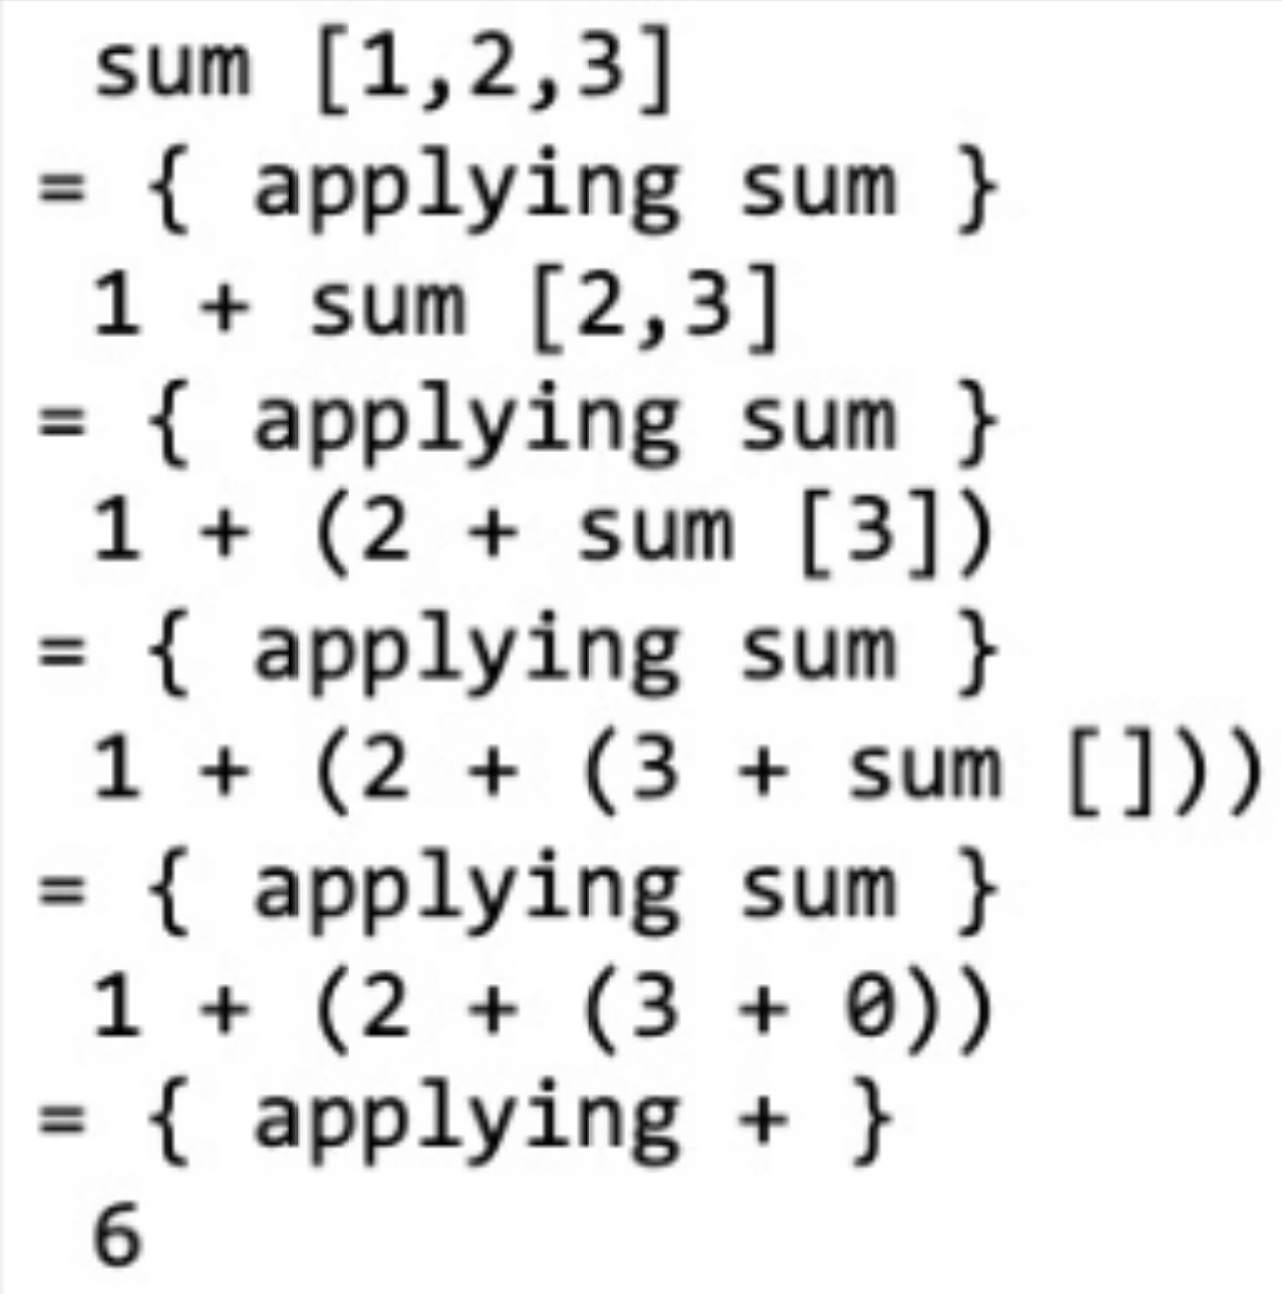
\includegraphics[width=0.5\textwidth]{resources/example1.PNG}
    \caption{Example 1}
\end{figure}
\begin{figure}
    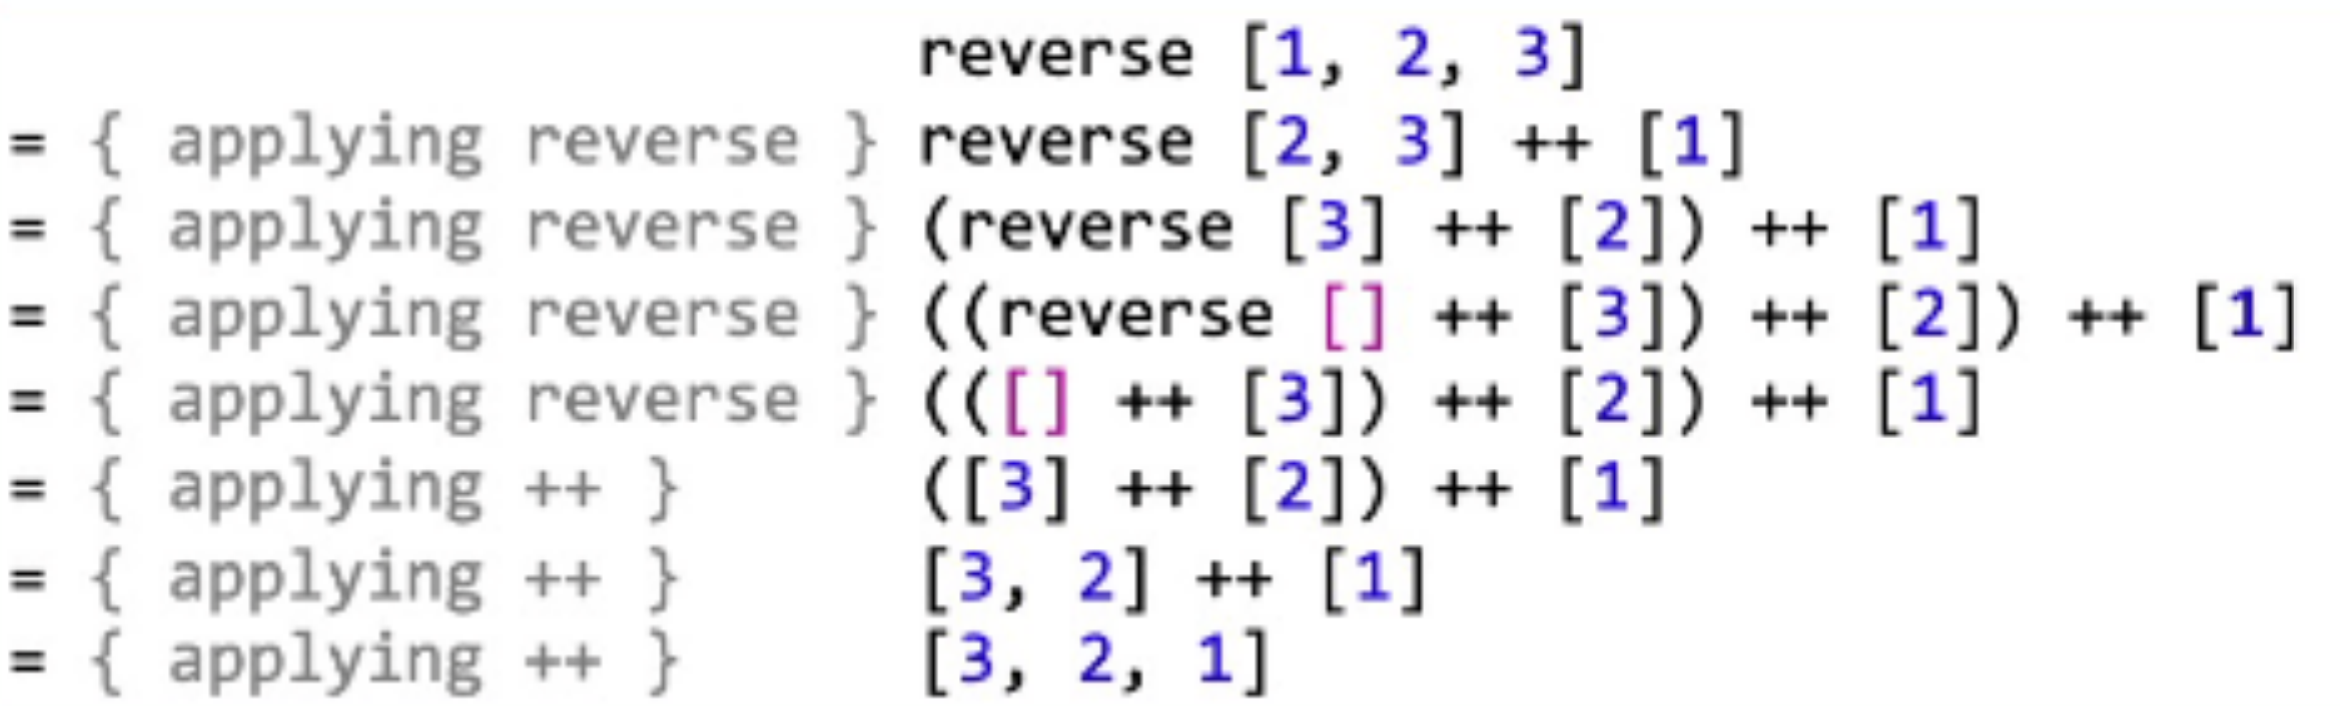
\includegraphics[width=1.0\textwidth]{resources/example2.PNG}
    \caption{Example 2}
\end{figure}
\begin{figure}
    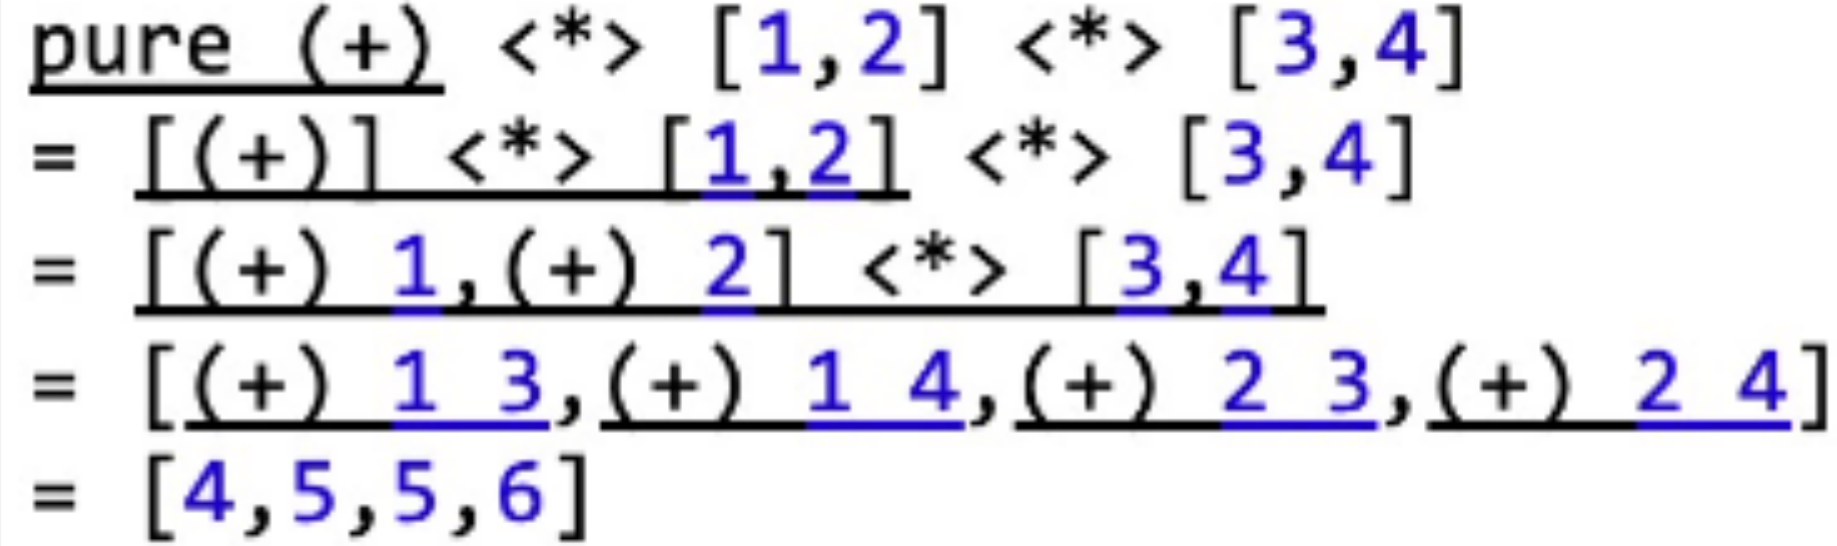
\includegraphics[width=0.75\textwidth]{resources/example3.PNG}
    \caption{Example 3}
\end{figure}
\begin{figure}
    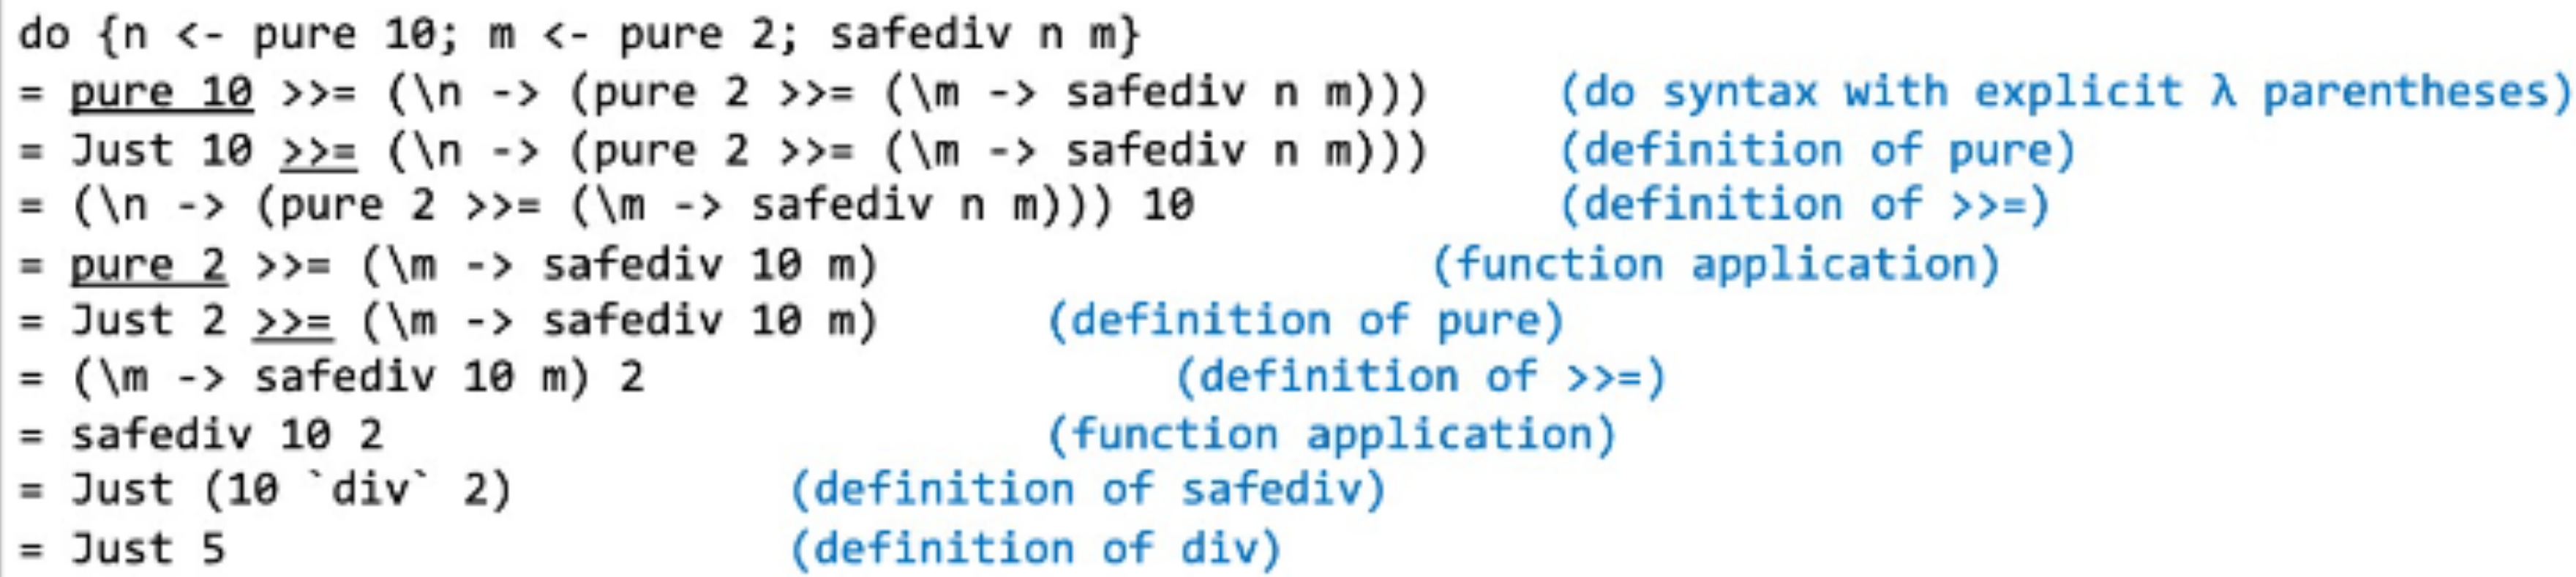
\includegraphics[width=1\textwidth]{resources/example4.PNG}
    \caption{Example 4}
\end{figure}
